\documentclass[../main.tex]{subfiles}
\begin{document}
\newpage
\section{Способы определения произведения рядов. Теорема Коши о перемножении абсолютно сходящихся рядов}

Для конечных сумм произведение определяется понятно: \( \left(\sum\limits_{ k=1}^{ K} a_k\right)\left( \sum\limits_{ j=1}^{ J} b_j\right)= \sum\limits_{ \substack{k=1 \ldots K\\ j=1 \ldots J}}^{ } a_kb_j\). 

Тогда произведением рядов должна быть сумма элементов такой бесконечной матрицы: 
\begin{equation*}
    \begin{pmatrix}
        a_1b_1 & a_1b_2 & a_1b_3 & \dots \\
        a_2b_1 & a_2b_2 & a_2b_3 & \dots \\
        a_3b_1 & a_3b_2 & a_3b_3 & \dots \\ 
        \vdots & \vdots & \vdots & \ddots
    \end{pmatrix}
\end{equation*}

Остаётся только вопрос: в каком порядке складывать?

\begin{center}
    \emph{Способы определения произведения рядов:} 
\end{center}

\begin{minipage}{0.5\textwidth}
    \begin{center}
        По квадратам

        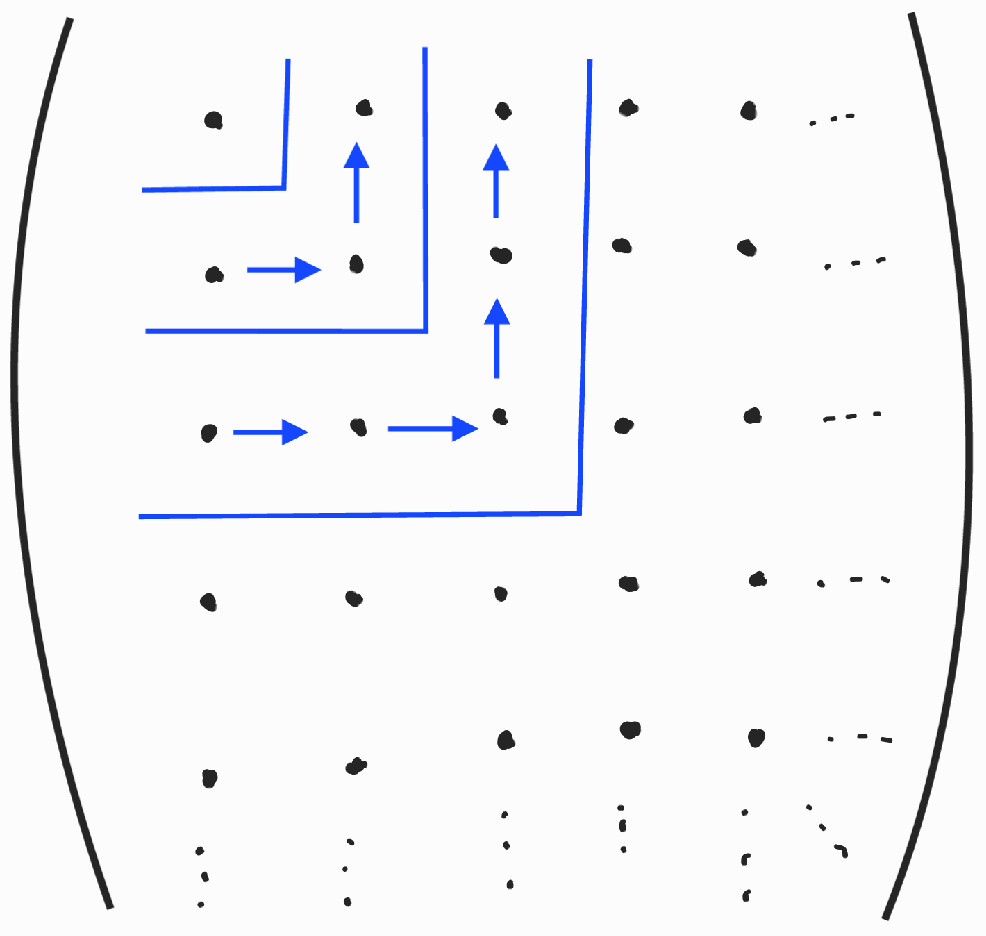
\includegraphics[width=0.65\linewidth]{59_squares.pdf}
    \end{center}
  \end{minipage}
  \begin{minipage}{0.5\textwidth}
    \begin{center}
        По Коши

        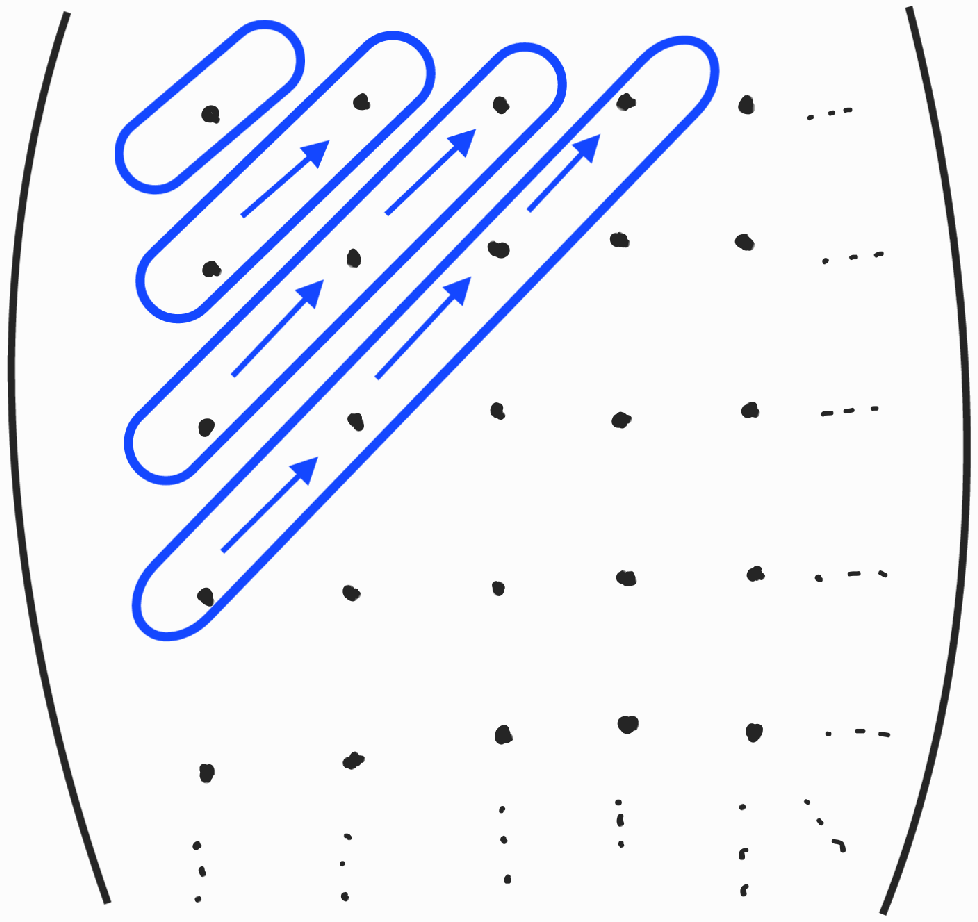
\includegraphics[width=0.65\linewidth]{59_koshi.pdf} 
    \end{center}
  \end{minipage}

\begin{thm}
    
    ~

    \( \Let \; \left\{ a_k\right\},\; \left\{ b_k\right\} \subset \C,\quad \sum\limits_{ k=1}^{ \infty } a_k,\; \sum\limits_{ k=1}^{ \infty } b_k\) сходятся абсолютно, \( \sum\limits_{ k=1}^{ \infty } p_k\) - ряд-произведение, полученный любым способом. 

    Тогда 
    \[ \sum\limits_{ k=1}^{ \infty } p_k \textrm{ сходится абсолютно и } \sum\limits_{ k=1}^{ \infty } p_k= \left( \sum\limits_{ k=1}^{ \infty } a_k\right) \left( \sum\limits_{ k=1}^{ \infty } b_k\right)\]
\end{thm}
\begin{proof}
    
    ~

    Достаточно только доказать, что ряд сходится абсолютно, потому что тогда \hyperlink{thm:series_transpose}{любая перестановка не меняет его сумму}, а ряды-произведения отличаются только перестановкой, при этом \hyperlink{thm:series_mul_squares}{ряд по квадратам имеет своей суммой \( \left( \sum\limits_{ k=1}^{ \infty } a_k\right) \left( \sum\limits_{ k=1}^{ \infty } b_k\right)\).}

    Пусть \( i, j: \N \longrightarrow \N\) - биекции, \( p_k = a_{i\left( k\right)}b_{j\left( k\right)}\). Обозначим \( \sum\limits_{ k=1}^{ \infty } a_k=A,\quad \sum\limits_{ k=1}^{ \infty } b_k=B\).

    \begin{equation*}
        \begin{aligned}
            \sum\limits_{ k=1}^{ n } \left| p_k\right|= \sum\limits_{ k=1}^{ n} \left| a_{i\left( k\right)}b_{j\left( k\right)}\right|= \sum\limits_{ k=1}^{ \infty } \left| a_{i\left( k\right)}\right|\left| b_{j\left( k\right)}\right| \leq \left( \sum\limits_{ p=1}^{ \max\limits_{ k=1 \ldots n}i\left( k\right) } \left| a_p\right| \right) \left( \sum\limits_{ q=1}^{ \max\limits_{ k=1 \ldots n} j\left( k\right)} \left| b_q\right|\right) \leq A\cdot B
        \end{aligned}
    \end{equation*}

    Ряд \( \sum\limits_{ k=1}^{ \infty } \left| p_k\right|\) ограничен, его общий член неотрицателен \( \Longrightarrow \sum\limits_{ k=1}^{ \infty } \left| p_k\right|\) сходится, то есть \( \sum\limits_{ k=1}^{ \infty } p_k\) сходится абсолютно. 
\end{proof}

\end{document}
